\chapter{Avaliação dos Segmentadores}\label{cap-segmentadores}



% =========== Avaliação dos Segmentadores ============ %
% \subsection{Avaliação dos Segmentadores}

\section{Preparação de um corpus de referência}

% ----- Segmnetação de Referência -----
A avaliação de um segmentador automático de textos exige uma referência, isto é, um conjunto de textos com os limites entre os segmentos conhecidos. Essa referência, deve ser confiável, sendo uma segmentação legítima que é capaz de dividir o texto em porções relativamente independentes, ou seja, uma segmentação ideal.


% ----- Anotação -----
Selecionou-se um grupo de anotadores para analisar e coletar dados referentes a segmentação de cada ata. O grupo de anotadores foi formado por profissionais com alguma afinidade com atas de reunião, como profissionais administrativos, professores e coordenadores de curso. Optou-se por desenvolver um \textit{software} como ferramenta para a coleta dos dados a fim de facilitar o trabalho de anotação e diminuir eventuais erros, conforme sugerido por~\cite{Hovy2010}. Essa ferramenta foi modelada para permitir aos anotadores visualizar os documentos e indicar livremente as divisões entre segmentos, bem como rotulá-los em classes e indicar palavras que melhor descrevem o assunto central do segmento.
Os anotadores receberam informações básicas sobre o objetivo da pesquisa e instruções de como operar o \textit{software}. Contudo, nenhum critério foi estabelecido para o procedimento ficando os anotadores livres para segmentar e rotular as atas orientados apenas pela interface da ferramenta. Na Figura~\ref{fig:interfaceanotacoes} é mostrada a interface da ferramenta utilizada para as anotações.

  \begin{figure}[!h]
	  \centering
	  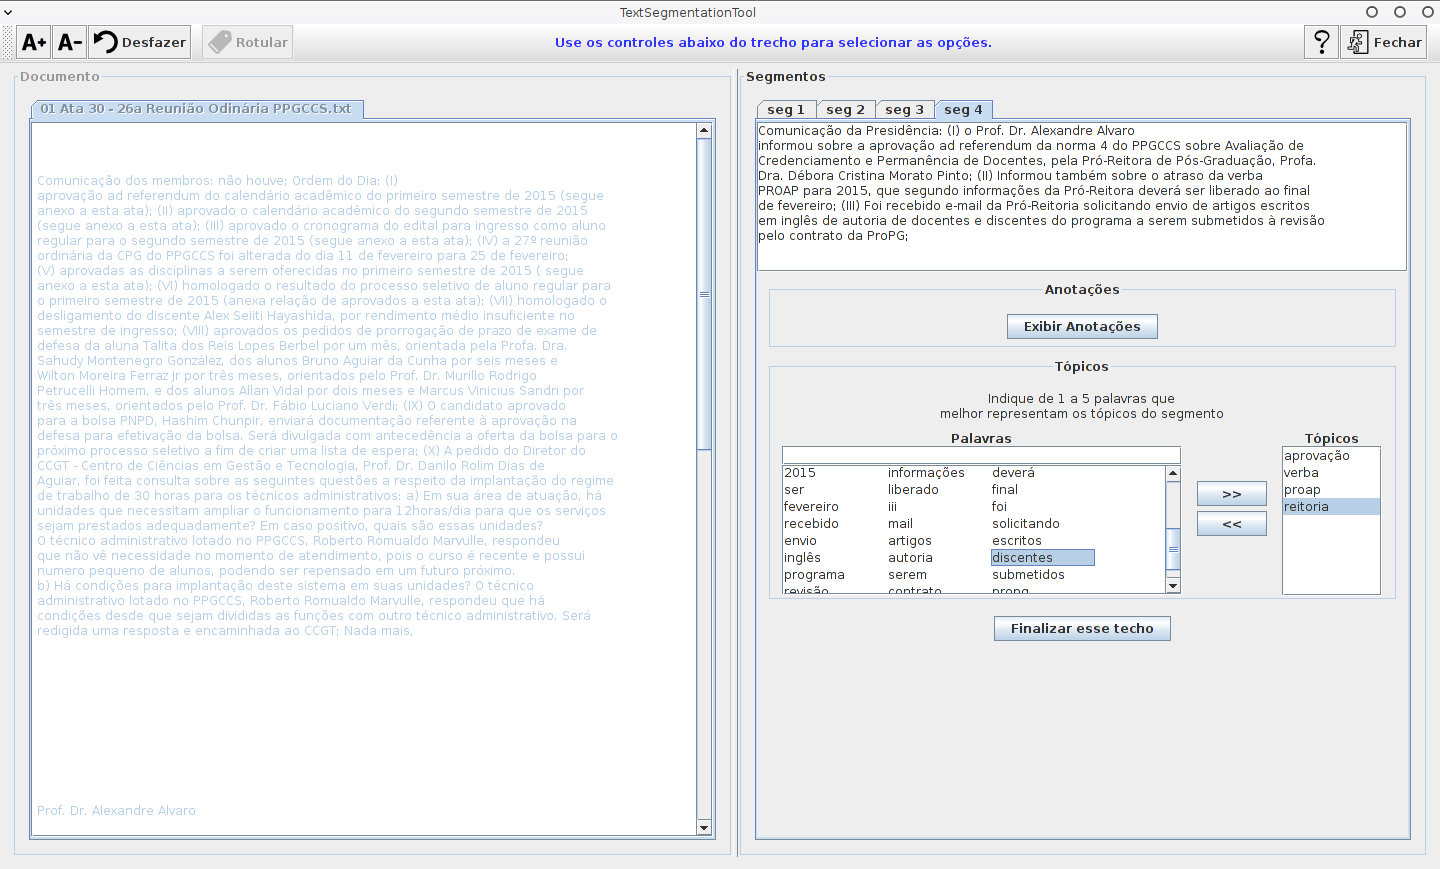
\includegraphics[width=1\textwidth]{conteudo/capitulos/figs/interface-anotacoes.png}
	  \caption{Interface da ferramenta utilizada para anotações onde o texto a ser segmentado é exibido no painel a esquerda e os controles para anotação estão disponíveis a direita.}
	  \label{fig:interfaceanotacoes}
  \end{figure}




% ----------------- Exemplo Segmentação de Referência ----------------------

Na Tabela~\ref{tab:segmentacaoreferencia} é mostrado um exemplo em que 6 dos 9 anotadores concordaram a respeito de um segmento. O trecho mostra quatro segmentos extraídos da segmentação de referência. 
%O primeiro trata ...
Cada linha contém um sentença os números a esquerda indicam seu índice e os segmentos estão separados por uma linha horizontal.

Anexo a cada segmento é mostrado a classe uma amostra das classes e descritores rotulados por um dos anotadores. Esses rótulos não foram utilizados no processo de segmentação e não têm nenhuma influência sobre a segmentação de referência. Nesse trabalho, essas anotações são utilizadas na avaliação dos extratores de tópicos e do Módulo de consulta.

\begin{table}[!h]
	\centering 
\footnotesize
% \scriptsize
	\begin{tabular}{|p{0.2cm}p{14,5cm}|} \hline


$^{[7]}$&
(II) Encerrada a etapa de inscrição para o processo seletivo como aluno regular para o segundo semestre de 2015: foram quarenta e nove inscrições on-line e dezoito candidatos entregaram a documentação; 
\textit{<informe>} \textit{<processo;seletivo>}
\\ \hline


$^{[8]}$ &
(III) O Prof. Dr. AAA informou que a Pró-Reitora comunicou a oferta de mais uma bolsa pela cota da Pró-Reitoria, mas não havia aluno disponível para alocação da bolsa.\\
$^{[9]}$ &
(III) O Prof. Dr. AAA informou que a Pró-Reitora comunicou a oferta de mais uma bolsa pela cota da Pró-Reitoria, mas não havia aluno disponível para alocação da bolsa.\\
$^{[10]}$ &
O Prof. Dr. BBB informou que havia uma aluna interessada, mas não informada durante o processo de elaboração do ranking no início do semestre.\\
$^{[11]}$ &
Ficou decidido enviar e-mail aos docentes solicitando que comuniquem permanentemente interesse de alunos em bolsa pra atualização do ranking;
\textit{<informe>} \textit{<solicitação;bolsa;cota;ranking;alunos>}
\\ \hline


$^{[12]}$ &
(IV) Com a mudança do Prof. Dr. DDD para o campus de São Carlos, o Prof. Dr. BBB assume o posto de suplente da linha Teoria Aplicada à Computação na CPG;
\textit{<informe>} \textit{<mudança;suplente;teoria;aplicada;computação>}
\\ \hline

$^{[13]}$ &
	Comunicação dos membros: Não houve;
	\textit{<irrelevante>} 
\\ \hline



% $^{[14]}$ &
% Ordem do Dia: (I) Foram apresentadas regras para participação de membro externo em banca de defesa do mestrado.\\
% $^{[15]}$ &
% O Prof. Dr. Alexandre Alvaro comentou que está sendo pago aos participantes externos das bancas a diária pelo PROAP e o pró-labore pelo DComp, além do programa fornecer o transporte, que onera a verba PROAP.\\
% $^{[16]}$ &
% O Prof. Dr. Tiago Agostinho de Almeida sugeriu o seguinte cálculo para pagamento: se o participante vier de uma Instituição com distância até 220 km será feito o cálculo de R\$ 1,00 multiplicado pela quilometragem.\\
% $^{[17]}$ &
% Caso a distância seja superior a 220 km, será calculada a distância multiplicada por R\$ 0,60. O menor valor entre o custo do transporte e o pagamento de verba e pró-labore será utilizado para custear a vinda do participante;
% \\ \hline



% $^{[18]}$ &
% (II) Foi discutida a forma de convalidação de disciplinas cursadas como aluno regular anterior a três anos do reingresso do aluno.
% Foi decidido que fica a cargo da CPG decidir sobre as disciplinas que serão aproveitadas quando do reingresso do aluno;
% \\ \hline



% $^{[13]}$ &

	\end{tabular}
	\caption{Exemplo de segmentação de referência com rotulação de um anotador}
	\label{tab:segmentacaoreferencia}
\end{table}









  
% Os arquivos gerados foram tratados para que os segmentos sempre terminem em uma sentença reconhecida pelo algoritmo, uma vez que as sentenças são a unidade mínima de informação nesse trabalho.
  Após o processo de anotação, os dados coletados foram analisados para gerar as segmentações de referência. A segmentação de referência foi gerada utilizando o critério de maior concordância, como já relatado em outros trabalhos~\cite{Hearst1997, Cardoso2017, Kazantseva2012, Passonneau1997, Galley2003}. Considerou-se que ocorre um limite entre segmentos quando a maioria dos anotadores (metade mais um) concordaram que a mesma sentença é um final de segmento. A concordância entre os anotadores é uma medida importante que mostra como os anotadores compreendem os textos analisados e o nível de confiabilidade da segmentação de referência. Na Figura~\ref{fig:concordanciasegref} é mostrado um exemplo de criação de uma segmentação de referência por meio da concordância entre anotadores. As primeiras linhas representam segmentações fornecidas por anotadores e a última linha representa a segmentação resultante da concordânica entre a maioria dos segmentadores e portanto mais confiável. 

  \begin{center}
	\begin{figure}[h!]

	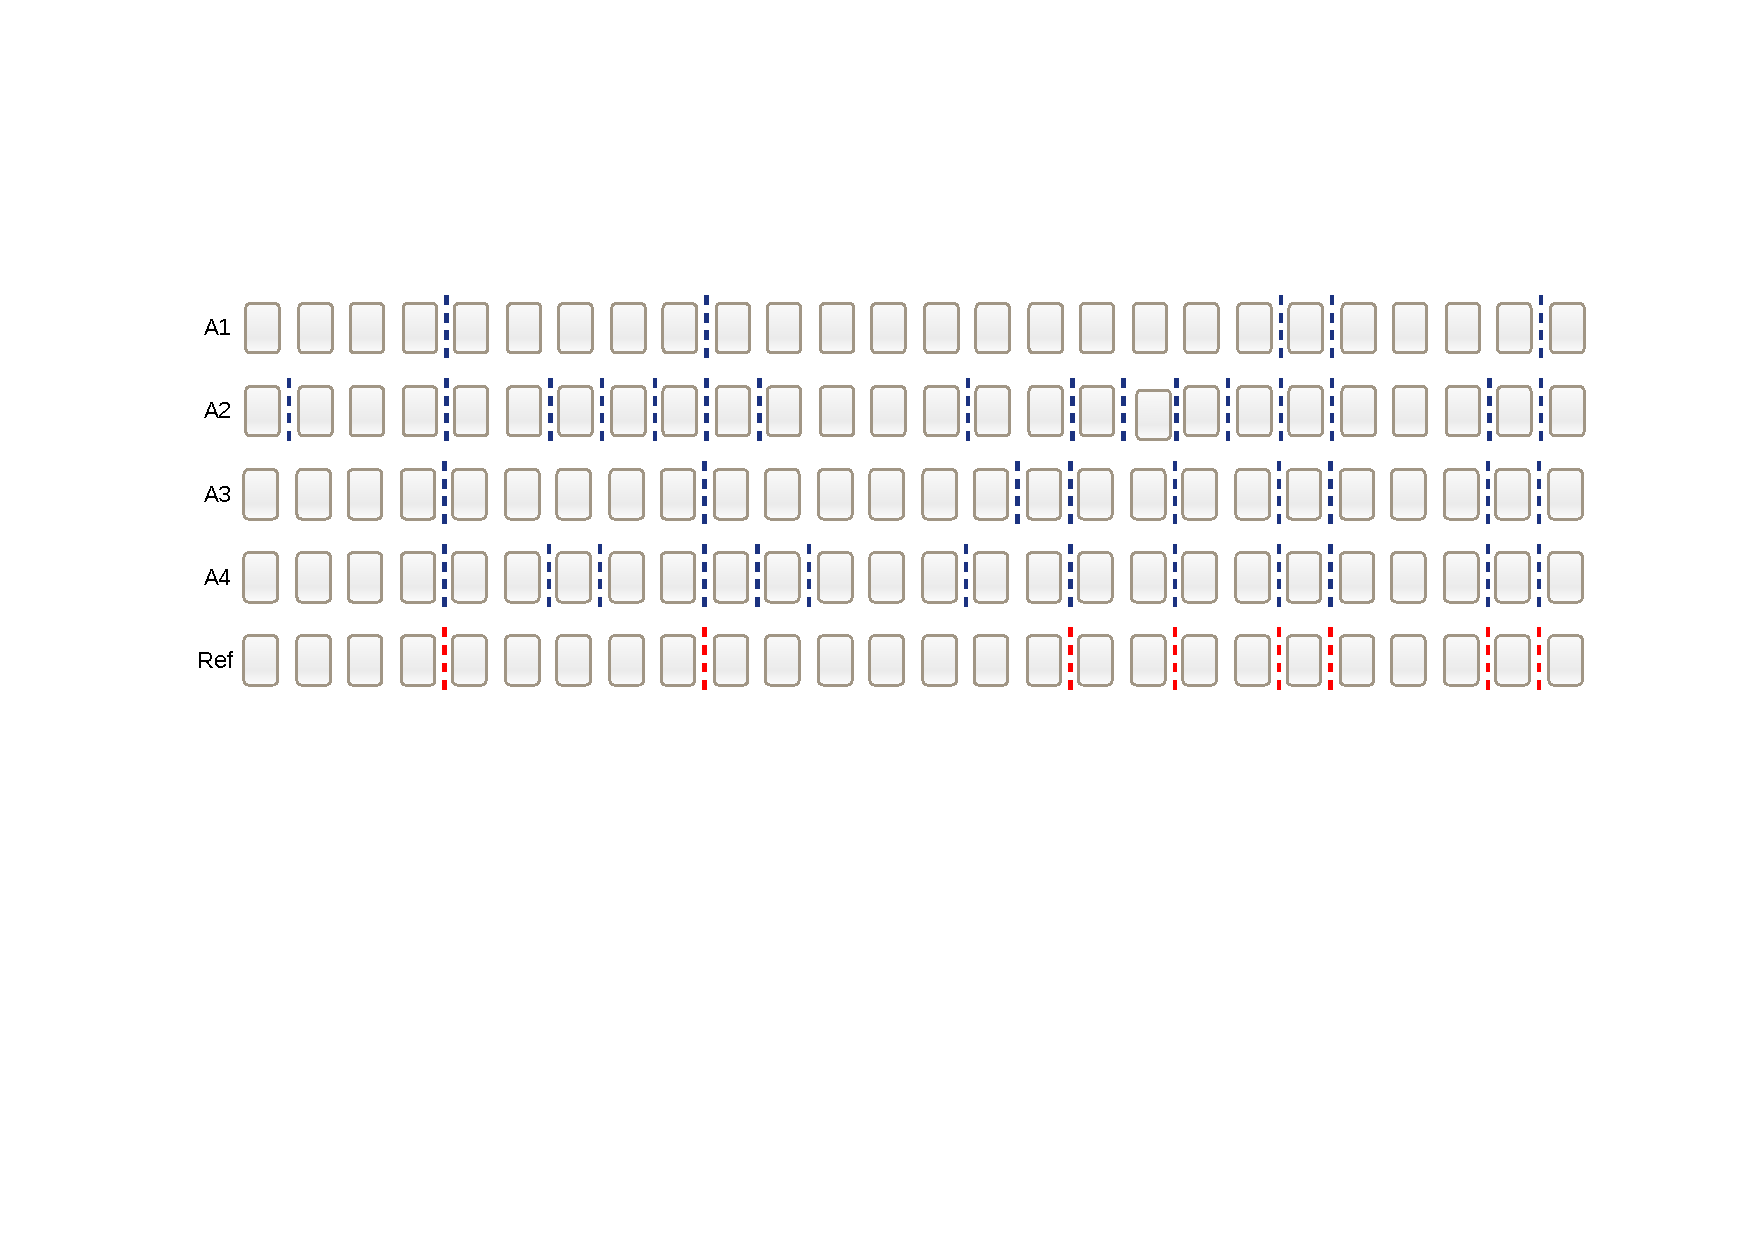
\includegraphics[trim={ 95 255 75 140 },clip,page=1,width=\textwidth]{conteudo/capitulos/figs/segmentacao-referencia.pdf}

	\caption{Exemplo uma segmentação de referência criada a partir da concordância entre segmentações manuais.}
	\label{fig:concordanciasegref}
	\end{figure}
\end{center}

Para mensurar a concordância entre anotadores, a medida \textit{kappa (k)}~\cite{Carletta1996} é frequentemente utilizada~\cite{Gruenstein2007, Cardoso2017, Hearst1997}. 
% Essa medida retorna um valor no intervalo de 0 até 1, onde 1 significa uma concordância perfeita e 0 que não houve concordância. 
Embora~\cite{Carletta1996} afirme que valores de k~>~0.8 indicam que os dados são confiáveis, visto a subjetividade da tarefa de segmentação textual, medidas menores podem ser aceitaveis, como reportado em~\cite{Hearst1997} que alcançou k~=~0,64 e~\cite{Cardoso2017}, k~=~0,56.  

A Tabela~\ref{tab:segmentacaoreferencia} contém, para cada ata, a quantidade de sentenças e a quantidade de segmentos identificadas pelos participantes.


\begin{table}[!h]
	\centering
	\begin{tabular}{|l|c|c|c|c|c|c|c|c|c|c|} \hline
		\textbf{Ata} & \textbf{Sentenças}  & 
		\textbf{A1}  & 
		\textbf{A2}  & 
		\textbf{A3}  & 
		\textbf{A4}  & 
		\textbf{A5}  & 
		\textbf{A6}  & 
		\textbf{A7}  & 
		\textbf{A8}  & 
		\textbf{A9} \\	\hline

% 		              A1   A2   A3  A4    A5   A6   A7   A8   A9   
		Ata 1  & 25 & 7  & 4  & 11 & 6  & 16 & 8  & 8  & 15 & 16 \\ \hline 
		Ata 2  & 17 & 4  & 4  & 8  & 6  & 11 & 6  & 6  & 15 & 14 \\ \hline 
		Ata 3  & 26 & 6  & 6  & 8  & 4  & 15 & 9  & 10 & 18 & 14 \\ \hline 
		Ata 4  & 26 & 5  & 5  & 10 & 6  & 14 & 17 & 7  & 11 & 12 \\ \hline 
		Ata 5  & 33 & 4  & 4  & 6  & 5  & 17 & 22 & 9  & 18 & 16 \\ \hline 
		Ata 6  & 11 & 3  & 4  & 6  & 4  & 9  & 9  & 4  & 7  &  5 \\ \hline 
		Ata 7  & 20 & 3  & 7  & 5  & 4  & 11 & 14 & 5  & 5  &  4 \\ \hline 
		Ata 8  & 35 & 4  & 8  & 3  & 8  & 12 & 17 & 5  & 11 &  9 \\ \hline 
		Ata 9  & 24 & 3  & 5  & 3  & 6  & 11 & 11 & 3  & 9  &  9 \\ \hline 
		Ata 10 & 50 & 4  & 5  & 4  & 7  & 31 & 29 & 5  & 9  &  8 \\ \hline 
		Ata 11 & 43 & 4  & 7  & 5  & 7  & 29 & 19 & 5  & 9  & 12 \\ \hline 
		Ata 12 & 56 & 3  & 10 & 4  & 16 & 33 & 25 & 4  & 13 & 11 \\ \hline 

	\end{tabular}
	\caption{Quantidade de sentenças e segmentos de referência por ata.}
	\label{tab:segmentacaoreferencia}
\end{table}






\section{Configuração experimental}
\label{subsec:configuracaoexperimental}

  

% -> Parâmetros do TT
O \textit{TextTiling} permite ajustarmos dois parâmetros, sendo o tamanho da janela e o passo. Por meio de testes empíricos escolheu-se os valores os valores 20, 40 e 60 para o tamanho da janela e 3, 6, 9 e 12 para o passo. Gerando ao final 20 configurações.
%

% -> Parâmetros do C99
O \textit{C99} permite o ajuste de três parâmetros, sendo, o primeiro a quantidade segmentos desejados, uma vez que, não se conhece o número ideal de segmentos e os documentos não apresentam muitos candidatos, calculou-se uma proporção dos candidatos a limite. Para isso atribuiu-se os valores {0,2; 0,4; 0,6; 0,8}. Para o segundo parâmetro, o tamanho do quadro utilizado para gerar a matriz de ranking, atribuiu-se os valores 9 e 11, sendo 11 o valor padrão da apresentado pelo autor. O algoritmo permite ainda indicar se as sentenças serão representados por vetores contendo a frequência ou o peso de cada termo. Ambas as representações foram utilizadas. Considerando todos os parâmetros, foram geradas 16 configurações para o algoritmo \textit{C99}.

Os algoritmos tradicionais baseados em coesão léxica como o \textit{TextTiling} e \textit{C99} são fortemente afetados pela distribuição das palavras no texto, pois a maioria das medidas de similaridade baseiam-se na frequência das palavras. Para esses, a remoção de termos menos significativo na etapa de pré-processamento pode influenciar o desempenho. Para outras abordagens como \textit{MinCutSeg} e \textit{BayesSeg} usou-se as configurações fornecidas por~\cite{Eisenstein2008}, onde essas técnicas foram utilizadas como \textit{base line}. Para \textit{TextSeg} não requer configuração de parâmetros.
Há ainda outras estratégias passíveis de aplicação, como a utilização de fontes externas, por exemplo \textit{thesaurus} e palavras pista, como discutido em \cite{Naili2016, Gutierrez2016, Ferret2009}. Nesse trabalho, essas estratégias não são utilizadas para manter uma abordagem não supervisionada e independente de domínio. 
% evitar a necessidade de  
	

\section{Critérios de avaliação}

% -> Definição do que é um bom algoritmo de segmentação
Para fins de avaliação desse trabalho, um bom método de segmentação é aquele cujo resultado melhor se aproxima de uma segmentação de referência, sem a obrigatoriedade de estar perfeitamente alinhado com tal. Ou seja, visto o contexto das atas de reunião, e a subjetividade da tarefa, não é necessário que os limites entre os segmentos (real e hipótese) sejam idênticos, mas que se assemelhem em localização e quantidade.

Os algoritmos foram comparados com a segmentação de referência obtida e calculou-se as medidas mais aplicadas à segmentação textual, $P_k$ e \textit{WindowDiff}. Além dessas, computou-se também as medidas tradicionais acurácia, precisão, revocação e $F^1$ para comparação com outros trabalhos que as utilizam.

% Inicialmente, 
Calculou-se as medidas configurando cada algoritmo conforme mostrado na Subseção~\ref{subsec:configuracaoexperimental}.  
A fim de conhecer o impacto do pré-processamento nos algoritmos \textit{TextTiling} e \textit{C99}. Esses foram testados em duas etapas: com o texto integral, e com o texto pré-processado em que elementos menos significativos foram removidos, conforme mencionado na Seção~\ref{sec:modulo-preparacao}.  
O teste de Friedman foi utilizado para gerar um ranking das melhores configurações para cada medida calculada. Com isso, foi possível descobrir quais valores otimizam um algoritmo para cada medida, considerando seus parâmetros e a influência do pré-processamento. 
 
Como já mencionado, os algoritmos \textit{MinCutSeg}, \textit{TextSeg} e \textit{BayesSeg} aplicou-se a etapa de pré-processamento e foram testados com as configurações apresentadas por~\cite{Eisenstein2008}. 










\section{Resultados}


Obteve-se, por meio dos testes apresentados, as melhores configurações para as principais medidas de avaliação de segmentadores. Com essas configurações calculou-se a média de cada medida considerando o conjunto de documentos. 


A seguir são apresentados os resultados obtidos com os algoritmos baseados em coesão léxica, considerando seus principais parâmetros e a aplicação do pré-processamento. Em seguida, são apresentados os resultados da avaliação final dos algoritmos abordados nesse trabalho.


Na Tabela~\ref{tab:resultadosTT} são apresentadas, as médias obtidas com o \textit{TextTiling} bem como as configurações utilizadas, onde \textbf{J} é o tamanho da janela e \textbf{P} é o passo.


\begin{table}[!h]
	\centering
	\begin{tabular}{|l||c|c|c||c|c|c|} \hline

		& \multicolumn{3}{c||}{Sem Pré-processamento} 
		& \multicolumn{3}{c|}{Com Pré-processamento}\\			

		\textbf{Medida} & 
		\textbf{J} &
		\textbf{P} & 
		\textbf{Média} &
		\textbf{J} &
		\textbf{P} & 
		\textbf{Média} \\	\hline

		P$_k$				& 50 & 9 & 0,142 & 50 & 9  & 0,144 \\ \hline
		\textit{WindowDiff}	& 50 & 6 & 0,387 & 40 & 9  & 0,396 \\ \hline
		Acurácia			& 50 & 6 & 0,612 & 40 & 9  & 0,603 \\ \hline
		Precisão			& 40 & 9 & 0,611 & 50 & 12 & 0,613 \\ \hline
		Revocação			& 20 & 3 & 0,886 & 20 & 3  & 0,917 \\ \hline
		F$^1$				& 30 & 6 & 0,605 & 40 & 3  & 0,648 \\ \hline

	\end{tabular}
	\caption{Resultados obtidos com o \textit{TextTiling}}
	\label{tab:resultadosTT}
\end{table}




%%%%%%%%%%%%%%%%%%%%%%
% Análise da Coesão Léxica e eficiência da técnica do TT
%%%%%%%%%%%%%%%%%%%%%%

% --> Falar da coesão léxica peculiar das atas!!

Uma vez que a coesão léxica é pressuposto de muitas abordagens em segmentação textual, fez-se uma análise desses documentos quanto a similaridade dos termos ao longo do texto. Verificou-se que a técnica de janelas deslizantes empregada pelo TextTiling encontra os vales que indicam transições entre segmentos, contudo ao comparar esses vales com a segmentação de referência, nota-se que a maioria dos limites coincide  ou estão próximos aos vales, porém há casos onde a referência indica limites em trechos com alta coesão léxica e outros onde a queda da coesão, indicada por vales, não coincide com nenhum limite de referência. 



% Na Figura~\ref{fig:coesaolexicaTT}a linha horizontal representa a variação da coesão léxica ao longo de uma ata e as linha verticais azuis e vermelhas representam os limites entre segmentos atribuidos pela referência e pelo algoritmo respectivamente. 
Na Figura~\ref{fig:coesaolexicaTT} é apresentado a variação da coesão léxica ao longo de uma ata e a segmentação obtida pelo \textit{TextTiling} usando tamanho de janela igual a 50 e passo 9. A linha horizontal representa a variação da coesão léxica e as linha verticais azuis e vermelhas representam os limites entre segmentos atribuídos pela referência e pelo algoritmo respectivamente. 





  %--- ---
  \begin{figure}[!h]
	  \centering
	  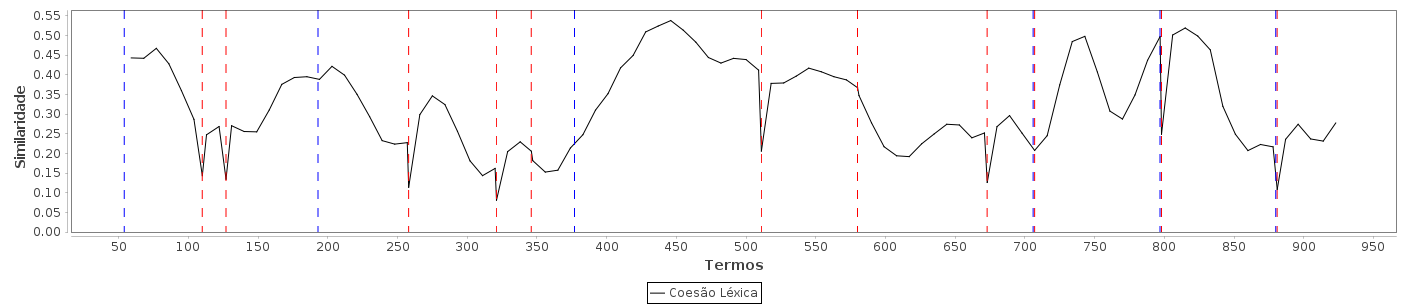
\includegraphics[width=\textwidth]{conteudo/capitulos/figs/coesaolexicaTT-50-9.png}
	  \caption{Variação da coesão léxica ao longo de uma ata junto a uma segmentação automática em contraste com uma segmentação de referência.}
	  \label{fig:coesaolexicaTT}
  \end{figure}




Na Tabela~\ref{tab:resultadosc99} são apresentadas, as médias obtidas com o \textit{C99} bem como as configurações utilizadas, onde \textbf{S} é a proporção de segmentos em relação a quantidade de candidatos, \textbf{M} é o tamanho do quadro utilizado para criar a matriz de \textit{rankings} e \textbf{W} indica se os segmentos são representados por vetores contendo a frequência ou um peso das palavras.


\begin{table}[!h]
	\centering
	\begin{tabular}{|l||c|c|c|c||c|c|c|c|} \hline

		& \multicolumn{4}{c||}{Sem Pré-processamento} 
		& \multicolumn{4}{c|}{Com Pré-processamento}\\			

		\textbf{Medida} & 
		\textbf{S} & 
		\textbf{M} & 
		\textbf{W} & 
		\textbf{Média} &
		\textbf{S} & 
		\textbf{M} & 
		\textbf{W} & 
		\textbf{Média} \\	\hline

		P$_k$				& 20 & 9 & Sim & 0,134& 20 & 11 & False	& 0,116 \\ \hline  
		\textit{WindowDiff}	& 60 & 9 & Sim & 0,411& 60 &  9 & Sim 	& 0,390 \\ \hline  
		Acurácia			& 60 & 9 & Sim & 0,588& 60 &  9 & Sim 	& 0,609 \\ \hline  
		Precisão			& 40 & 9 & Sim & 0,645& 20 & 11 & False	& 0,720 \\ \hline  
		Revocação			& 80 & 9 & Sim & 0,869& 80 & 11 & Sim 	& 0,897 \\ \hline  
		F$^1$				& 80 & 9 & Sim & 0,638& 80 & 11 & Sim 	& 0,655 \\ \hline  

	\end{tabular}
	\caption{Resultados obtidos com o \textit{C99}}
	\label{tab:resultadosc99}
\end{table}



Verificou-se que, entre os métodos baseados em coesão léxica, o \textit{C99} obteve melhor desempenho em acurácia, precisão, $F^1$, $P_k$ e \textit{WindowDiff}, em relação ao \textit{TextTiling}, enquanto este obteve o melhor desempenho em revocação. De maneira geral, o algoritmo \textit{C99} apresenta melhores resultados em relação ao \textit{TextTiling}, contudo testes estatísticos realizados indicaram que não houve diferença significativa entre os métodos. 



% --> colocar os CDs aqui?

Com os testes anteriores obteve-se, para cada medida, 4 configurações levando em conta ambos os algoritmos e a presença ou ausência do pré-processamento. Por meio do teste de Friedman e Nemenyi e verificou-se que não há diferença crítica entre os métodos \textit{TextTiling} e \textit{C99}. Na Figura~\ref{fig:CDs} é mostrado os Diagramas para as medidas \textit{WindowDiff}, $P_k$, Acurácia, Precisão, Revocação e $F^1$.	

\begin{figure}[!h]
	\centering     %%% not \center

	\subfigure[a]{ \label{fig:a}
		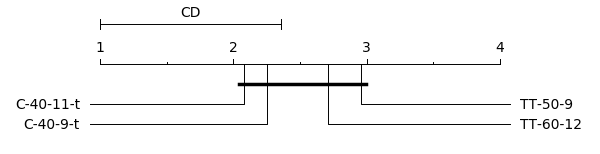
\includegraphics[width=70mm]{conteudo/capitulos/figs/CDs/WinDiff.png} }	
	\subfigure[b]{ \label{fig:b}
		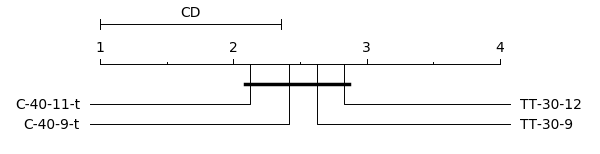
\includegraphics[width=70mm]{conteudo/capitulos/figs/CDs/Pk.png} }
	\subfigure[c]{ \label{fig:c}
		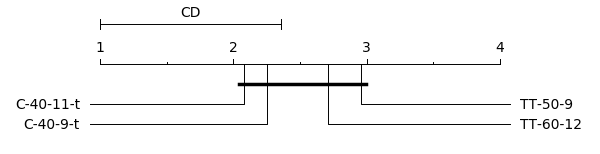
\includegraphics[width=70mm]{conteudo/capitulos/figs/CDs/Acuracy.png}}
	\subfigure[d]{ \label{fig:d}
		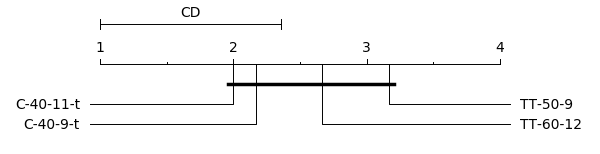
\includegraphics[width=75mm]{conteudo/capitulos/figs/CDs/Precision.png}}
	\subfigure[e]{ \label{fig:e}
		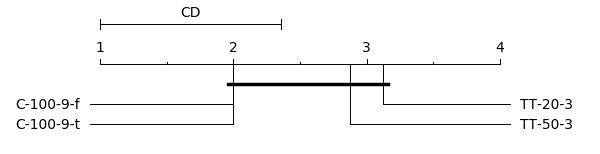
\includegraphics[width=70mm]{conteudo/capitulos/figs/CDs/Recall.png}}
	\subfigure[f]{ \label{fig:f}
		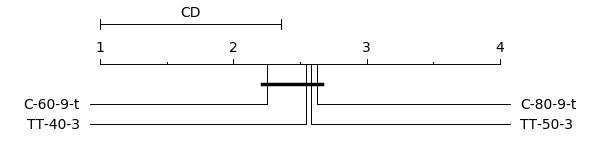
\includegraphics[width=70mm]{conteudo/capitulos/figs/CDs/F1.png}}

		\caption{Diagramas de Diferença Crítica sobre \textit{ranking} dos algoritmos de segmentação baseados em coesão léxica de acordo com valores de \textit{WindowDiff}, $P_k$, Acurácia, Precisão, Revocação e $F^1$.}
	\label{fig:CDs}
\end{figure}
% -< Colocar uma explicação mais detalhada para esses passos
% --> Fechar falando sobre os métodos baseados em coesão léxica.


A avaliação final foi feita pela comparação dos algoritmos usando as medidas \textit{Pk} e \textit{WindowDiff}. É apresentada também, para fins de comparação, as medidas tradicionais acurácia, precisão, revocação e F$^1$, entretanto, nesse contexto, essas medidas são menos significativa que Pk e WindowDiff, conforme já mencionado na Seção~\ref{subsec:medidas-segmentacao}. A Tabela~\ref{tab:configfinal} contém as médias com cada algoritmo. Vale lembrar que P$_k$ e \textit{WindowDiff} são medidas de dissimilaridade, ou seja, os valores menores significam melhores resultados.

\begin{table}[!h]
	\centering
\begin{tabular}{|l||c|c|c|c|c|c|c|} 
\hline 
\textbf{M\'{e}todo} & 
\textbf{Pk} & 
\textbf{WD} & 
\textbf{A } & 
\textbf{P } & 
\textbf{R } & 
\textbf{F1} & 
\textbf{Segmentos}\\ \hline

Senten\c{c}as & 0.320 & 0.502 & 0.498 & 0.498 & \textbf{1.000} & \textbf{0.642} & 22.083\\ \hline
TextTiling    & 0.275 & 0.469 & 0.531 & 0.514 & 0.937 & 0.640 & 19.583\\ \hline
C99           & 0.142 & 0.426 & 0.574 & 0.601 & 0.473 & 0.506 & 8.167\\ \hline
BayesSeg      & 0.148 & 0.414 & 0.586 & 0.599 & 0.526 & 0.528 & 8.750\\ \hline
MinCut        & 0.226 & 0.532 & 0.468 & 0.464 & 0.438 & 0.432 & 10.333\\ \hline
TextSeg       & \textbf{0.085} & \textbf{0.387} & \textbf{0.613} & \textbf{0.714} & 0.412 & 0.497 & 5.167\\ \hline
\end{tabular} 

	\caption{Melhores resultados obtidos.}
	\label{tab:configfinal}
\end{table}


Na Figura~\ref{fig:grafico-medidas-tradicionais} é apresentada a performance dos algoritmos nas medidas tradicionais. Observa-se valores altos de revocação para a segmentação por sentenças, pois é atribuído um limite a todo candidato a final de segmento, o que resulta no valor máximo para revocação. De maneira semelhante, o comportamento do \textit{TextTiling} gera 
mais segmentos em relação aos demais, e com isso tem-se valores maiores de revocação, o que pode ser contornado configurando o algoritmo com passos maiores, ou ainda, sobre-escrevendo a função que calcula os \textit{depth scores} para reconhecer vales mais largos.

%--> TODO: explicar (a conceituação teórica) que passos curtos geram mais segmentos

  \begin{figure}[!h]
	  \centering
	  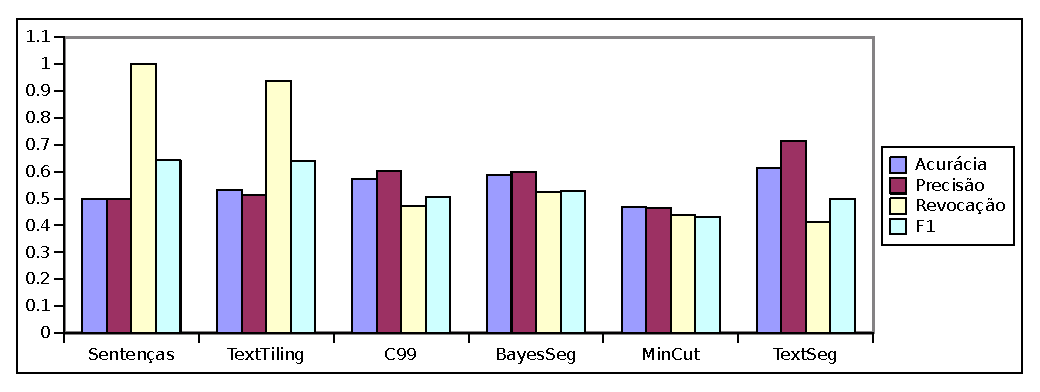
\includegraphics[width=1\textwidth]{conteudo/capitulos/figs/grafico-medidas-APRF1.eps}
	  \caption{Performance dos algoritmos de segmentação textual com as medidas tradicionais}
	  \label{fig:grafico-medidas-tradicionais}
  \end{figure}
  

Na Figura~\ref{fig:grafico-medidas-Pk-Wd} é apresentada a performance dos algoritmos nas medidas P$_k$ e \textit{WindowDiff}. Verifica-se que \textit{TextSeg} apresenta valores de \textit{WindowDiff} próximas ao \textit{C99} e \textit{BayesSeg} e resultados mais significantes quando medidos por P$_k$ em relação aos demais algoritmos.



  \begin{figure}[!h]
	  \centering
	  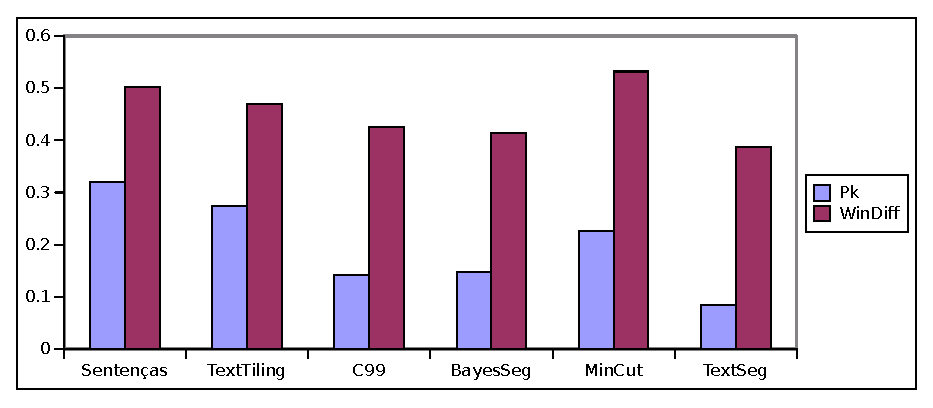
\includegraphics[width=1\textwidth]{conteudo/capitulos/figs/grafico-medidas-Pk-Wd.eps}
	  \caption{Performance dos algoritmos de segmentação textual com as medidas P$_k$ e \textit{WindowDiff}.}
	  \label{fig:grafico-medidas-Pk-Wd}
  \end{figure}




% De maneira geral, os métodos probabilísticos apresentam desempenho próximo 







% cada segmento é um documento
% Após a identificação dos segmentos, o algoritmo retorna uma lista onde cada elemento é um texto com um assunto predominante e será a partir de disso considerado um documento.
Após a identificação dos segmentos, o algoritmo retorna uma lista com fragmentos do texto original. Cada segmento é incorporado à estrutura de dados interna como subdocumentos com um tema relativamente independente. Em seguida, esses subdocumentos serão analisados pelo extrator de tópicos para identificação de descritores e agrupamento.









% -? Medidas

% -- como ele faz?






